% ----------------------------------------------------------------------------------------\
% ---------------------------------------------------------------------------------------\
% --------------------------------------------------------------------------------------\
\section{Análisis e interpretación de resultados}
% ----------------------------------------------------------------------------------------\
% ---------------------------------------------------------------------------------------\
% --------------------------------------------------------------------------------------\

% ----------------------------------------------------------------------------------------\
% ---------------------------------------------------------------------------------------\
\subsection{Diseño 1}
% ----------------------------------------------------------------------------------------\
% ---------------------------------------------------------------------------------------\
Después de definir la estructura de la red bayesiana y las tablas de probabilidad condicional (CPTs) correspondientes, el código verifica la validez del modelo y luego realiza una inferencia específica, la cual es la probabilidad de estar satisfecho con el trabajo bajo las siguientes condiciones:

\begin{itemize}
    \item Horas de trabajo: moderadas
    \item Balance trabajo-vida: equilibrado
\end{itemize}

Los resultados obtenidos son los siguientes:

\begin{lstlisting}
La probabilidad de estar satisfecho es:
+------------------------------------+-----------------------------+
| Satisfaccion laboral               |   phi(Satisfaccion laboral) |
+====================================+=============================+
| Satisfaccion laboral(satisfecho)   |                      0.8000 |
+------------------------------------+-----------------------------+
| Satisfaccion laboral(neutral)      |                      0.1500 |
+------------------------------------+-----------------------------+
| Satisfaccion laboral(insatisfecho) |                      0.0500 |
+------------------------------------+-----------------------------+
\end{lstlisting}

Estos resultados ilustran la dinámica entre el volumen de trabajo y el equilibrio entre la vida personal y laboral de la siguiente manera:

\begin{itemize}
    \item \textbf{Influencia directa de las horas de trabajo en la satisfacción laboral:}
    Las horas de trabajo moderadas pueden conducir a una mayor satisfacción laboral (0.8000 de probabilidad de estar satisfecho), mientras que un exceso de horas de trabajo podría disminuir la satisfacción laboral.

    \item \textbf{Importancia del balance trabajo-vida en la satisfacción laboral:}
    El balance trabajo-vida equilibrado también tiene un impacto significativo en la satisfacción laboral. Bajo condiciones de balance trabajo-vida equilibrado, incluso si las horas de trabajo son moderadas, la satisfacción laboral sigue siendo alta (0.8000 de probabilidad de estar satisfecho), esto resalta la importancia de no solo considerar las horas de trabajo, sino también cómo se equilibran con la vida personal para mantener una satisfacción laboral óptima.

    \item \textbf{Influencia indirecta de las horas de trabajo a través del balance trabajo-vida:}
    El balance trabajo-vida actúa como un mediador entre las horas de trabajo y la Satisfacción laboral, aunque las horas de trabajo pueden tener un impacto directo en la satisfacción laboral, este impacto puede ser mitigado o amplificado por el equilibrio entre la vida personal y laboral.
\end{itemize}


En resumen, este modelo resalta la importancia de mantener un balance saludable entre el trabajo y la vida personal para promover una mayor satisfacción laboral, muestra cómo las horas de trabajo y el equilibrio trabajo-vida interactúan entre sí para influir en la percepción de satisfacción en el trabajo, y enfatiza la necesidad de gestionar adecuadamente estas variables para mantener un entorno laboral saludable y productivo.


% ----------------------------------------------------------------------------------------\
% ---------------------------------------------------------------------------------------\
\subsection{Diseño 2}
% ----------------------------------------------------------------------------------------\
% ---------------------------------------------------------------------------------------\

Actualizar los packetes para no tener problemas 
\begin{itemize}
    \item \texttt{pip install --upgrade jupyter ipywidgets}
    \item \texttt{pip install --upgrade pgmpy}
\end{itemize}


% ---------------------------------------------------------------------------------------\
\subsubsection*{Comparación}
% ----------------------------------------------------------------------------------------\

Estos son los resultados de la primera red 
\begin{center}
    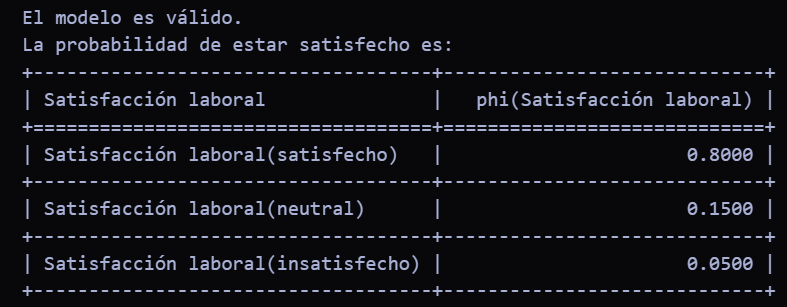
\includegraphics[scale = .6]{IMA/ejecucionRedBayesina.png}
\end{center}

Estos son los resultados de la red modificada incluyendo las variaciones de las horas de 
trabajo flexibles y la ayuda de IA dentro de las actividades del trabajo. 

\begin{center}
    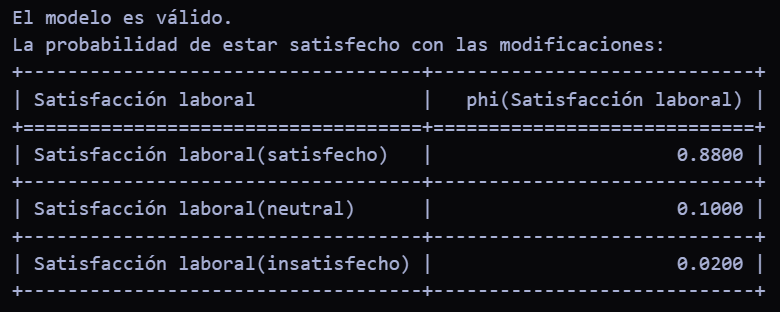
\includegraphics[scale = .6]{IMA/ejecucionRedModificada.png}
\end{center}

Observamos como se ha incrementado $88\%$ la la satisfacción lo que nos dice que las condiciones 
nuevas para el trabajo tienen un impacto positivo en la vida de los empleados. Para la 
respuesas neutrales respecto a su satisfacción en el trabajo es baja $10\%$  lo que podemos 
decir que pocas personas se sentiran en las mismas situciones con los dos cambios realizados, 
mientras que con un $2\%$ la probabilidad de insatisfacción es muy baja lo cual dice que las 
personas les gusta más poder tener un horario flexible desde casa y tener ayuda de la 
tecnología.

% ----------------------------------------------------------------------------------------\
% ---------------------------------------------------------------------------------------\
\subsection{Diseño 3}
% ----------------------------------------------------------------------------------------\
% ---------------------------------------------------------------------------------------\

Estos son los resultados de la primera red 
\begin{center}
    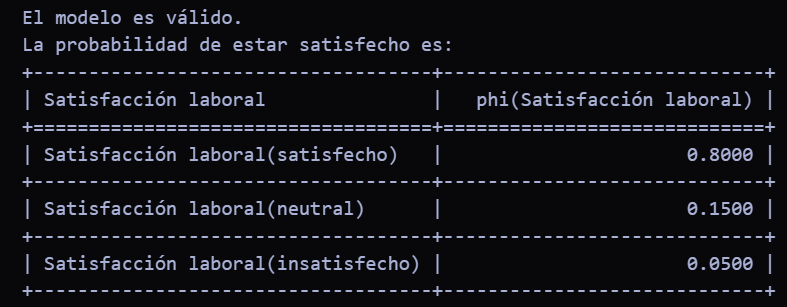
\includegraphics[scale = .6]{IMA/ejecucionRedBayesina.png}
\end{center}

Estos son los resultados de la red extendida, agregando el nodo de impacto del lider.

\begin{center}
    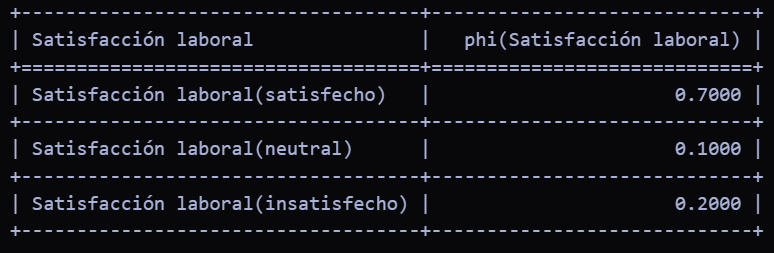
\includegraphics[scale = .6]{IMA/ejecucionRedExtension.png}
\end{center}

Vemos como ahora baja el porcentaje de estar satisfecho a un $70\%$ con nuestra 
variable del jefe. Así como tambien bajo la parte neutral de un $15\%$ a un 
$10\%$. Finalmente vemos como ahora es un $20\%$ la probabilidad de estar 
insatisfecho por el impacto que sienten los empleados cuadno no se tiene 
un jefe de calidad. 